\documentclass[tikz, border=15pt]{standalone}
\usetikzlibrary{positioning, shapes.gates.logic.US, calc}
\usepackage{amsmath}
\newcommand{\splitmark}[2]{(#1) node[circle, fill, inner sep= 0pt, outer sep= 0pt, minimum size= 2*#2]{}}

\begin{document}

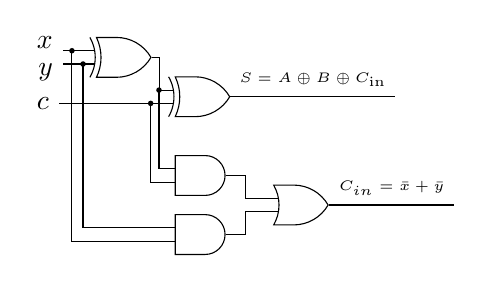
\begin{tikzpicture}
    %Gates
    \node[xor gate US, draw] (xor) at (1.0, -0.25) {};
    \node[xor gate US, draw] (xor2) at ((2.0, -0.75) {};
    \node[and gate US, draw] (and) at ($(xor2) + (0.0, -1.0)$) {};
    \node[and gate US, draw] (and2) at ($(and) + (0.0, -0.750)$) {};
    \node[or gate US, draw] (or) at ($ (and)!.5!(and2) + (1.25, 0.0)$) {};

    
    %Dot (connector)
    \draw (xor.input 1) -- \splitmark{[xshift=-8]xor.input 1}{1pt} |- (and2.input 2);
    \draw (xor.input 2) -- \splitmark{[xshift=-4]xor.input 2}{1pt} |- (and2.input 1);
    \draw (xor2.input 2) -- \splitmark{[xshift=-8]xor2.input 2}{1pt} |- (and.input 2);
    \draw (xor2.input 1) -- \splitmark{[xshift=-5]xor2.input 1}{1pt} |- (and.input 1);
    

    %Lines (Drawing Inputs)
    \draw (xor.input 1) -- node[at end,left, yshift=1mm]{$x$} ++(left:4mm);
    \draw (xor.input 2) -- node[at end,left, yshift=-1mm]{$y$} ++(left:4mm);    
    \draw (xor2.input 2) -- node[at end, left]{$c$} ++(left:1.45);


    %Lines (Drawing Outputs)
    \draw (xor.output) -- ($(xor) + (0.5, 0.0)$) |- (xor2.input 1);    
    \draw (and2.output) -- ($(and2)+(0.6,0.0)$) |- (or.input 2); 
    \draw (and.output) -- ($(and)+(0.6,0.0)$) |- (or.input 1); 


    %Boolean Functions
    \draw (or.output) -- node[above]{\tiny $C_{in} = \bar x + \bar y$} ($(or) + (2.0, 0)$);
    \draw (xor2.output) -- node[above]{\tiny $S = A \oplus B \oplus C_{\text{in}}$} ($(xor2)+ (2.5,0)$);
\end{tikzpicture}

\end{document}
